% ======================================================================
% Module 1: motivation, SEIRD model, published models, phase plane
% Four frames, no title slide: \input this file into the main deck.
%
% Needs in the main preamble:  \usepackage{graphicx,booktabs,amssymb,tikz}
%                              \usetikzlibrary{arrows.meta,positioning}
% Figures are in figs/ next to this file. If this file sits in a folder
% (e.g. module1/), add \graphicspath{{module1/}} to the main preamble.
% All numbers are from report/main.tex (final Colab run).
% ======================================================================

% Shared deck colours (same values as Module 5)
\definecolor{mvPINN}{HTML}{7B2D8E}
\definecolor{mvInk}{HTML}{1F2933}
\definecolor{mvMuted}{HTML}{5F6B7A}
\definecolor{mvSoft}{HTML}{F3EDF6}
\definecolor{mvRule}{HTML}{C9B6D3}

\providecommand{\mvTakeaway}[1]{%
  \par\vspace{3pt}\noindent
  \fcolorbox{mvRule}{mvSoft}{\parbox{\dimexpr\linewidth-2\fboxsep-2\fboxrule\relax}{\footnotesize\color{mvInk}#1}}}

% ----------------------------------------------------------------------
\begin{frame}{Why transmission must change over time}
\framesubtitle{Module 1 \textbullet\ Ebola in Sierra Leone, 2014--15 \textbullet\ an SEIRD model with a time-varying transmission rate $\beta(t)$}
\vspace{-2pt}
\begin{columns}[T,onlytextwidth]
\column{0.52\textwidth}
  \footnotesize\raggedright
  \textbf{\color{mvPINN}The problem}
  \begin{itemize}\setlength{\itemsep}{1pt}
    \item Ebola spreads by contact with body fluids, and with the dead at funerals
    \item isolation, safe burials and contact tracing cut transmission as the epidemic went on: $\beta$ is \textbf{not} a constant
    \item surveillance reports only cases and deaths; $S$ and $E$ are never measured
  \end{itemize}
  \vspace{4pt}
  \centering
  \begin{tikzpicture}[
      node distance=1.15cm,
      box/.style={rectangle, draw=mvPINN, fill=mvSoft, thick, minimum size=0.62cm,
                  font=\bfseries\small, rounded corners=2pt, text=mvInk},
      arr/.style={-{Stealth[length=2mm]}, thick, draw=mvInk!70}]
    \node[box] (S) {$S$};
    \node[box, right=of S] (E) {$E$};
    \node[box, right=of E] (I) {$I$};
    \node[box, right=of I] (R) {$R$};
    \node[box, below=0.55cm of I] (D) {$D$};
    \draw[arr] (S) -- node[above, font=\scriptsize] {$\beta(t)\,s\,i$} (E);
    \draw[arr] (E) -- node[above, font=\scriptsize] {$\sigma e$} (I);
    \draw[arr] (I) -- node[above, font=\scriptsize] {$\gamma i$} (R);
    \draw[arr] (I) -- node[right, font=\scriptsize] {$\mu i$} (D);
  \end{tikzpicture}\\[3pt]
  {\scriptsize $\dot s = -\beta s i,\;\; \dot e = \beta s i - \sigma e,\;\; \dot i = \sigma e - (\gamma+\mu) i,\;\; \dot r = \gamma i,\;\; \dot d = \mu i$\\[1pt]
  fractions of $N$, so $s+e+i+r+d = 1$ at all times}
\column{0.44\textwidth}
  \scriptsize\setlength{\tabcolsep}{4pt}
  \begin{tabular}{@{}lll@{}}
    \toprule
    & Meaning & Value \\
    \midrule
    $N$      & population (2014 census)  & 7{,}092{,}113 \\
    $\sigma$ & incubation rate (9.4 days) & 0.1064 /day \\
    $\gamma$ & recovery rate (7 days)     & 0.1429 /day \\
    $\mu$    & death rate                 & 0.1000 /day \\
    $\beta$  & transmission rate (baseline) & 0.4858 /day \\
    \midrule
    CFR      & $\mu/(\gamma+\mu)$          & 41.2\% \\
    $R_0$    & $\beta/(\gamma+\mu)$        & 2.00 \\
    \bottomrule
  \end{tabular}\\[5pt]
  \footnotesize
  \textbf{\color{mvPINN}Assumptions}
  \begin{itemize}\setlength{\itemsep}{0pt}
    \item closed population, homogeneous mixing
    \item recovered people stay immune
    \item $\sigma,\gamma$ fixed from WHO clinical data, so the data only have to determine $\beta(t)$ and $\mu$
  \end{itemize}
\end{columns}
\end{frame}

% ----------------------------------------------------------------------
\begin{frame}{Published models: how others handled $\beta(t)$}
\framesubtitle{Module 1 \textbullet\ each makes one assumption about how transmission changes, and each assumption has a cost}
\vspace{-2pt}
\begin{columns}[T,onlytextwidth]
\column{0.485\textwidth}
  \footnotesize\raggedright
  \textbf{\color{mvPINN}Chowell et al.\ (2004)} {\scriptsize\color{mvMuted}Congo 1995, Uganda 2000}
  \begin{itemize}\setlength{\itemsep}{0pt}
    \item SEIR model; $\beta$ is high until control begins, then falls
    \item fitted to case counts: $R_0 \approx 1.83$ (Congo), $1.34$ (Uganda)
    \item[$\times$] the \textbf{shape} of the fall is chosen in advance
  \end{itemize}
  \vspace{4pt}
  \textbf{\color{mvPINN}Legrand et al.\ (2007)} {\scriptsize\color{mvMuted}three routes of infection}
  \[ \lambda(t) = \beta_I \tfrac{I}{N} + \beta_H \tfrac{H}{N} + \beta_F \tfrac{F}{N} \]
  \vspace{-10pt}
  \begin{itemize}\setlength{\itemsep}{0pt}
    \item community ($I$), hospital ($H$) and funeral ($F$) transmission
    \item[$\times$] $H$ and $F$ follow $I$, so from one national case curve the three $\beta$'s trade off: \textbf{many sets fit equally well}
  \end{itemize}
\column{0.485\textwidth}
  \footnotesize\raggedright
  \textbf{\color{mvPINN}Rivers et al.\ (2014)} {\scriptsize\color{mvMuted}a policy step}
  \[ \beta(t) = \beta_0\,\big[1 - \delta\;\mathbf{1}(t \ge t_{\text{policy}})\big] \]
  \vspace{-10pt}
  \begin{itemize}\setlength{\itemsep}{0pt}
    \item $\beta$ drops by a fraction $\delta$ on a chosen date ($\mathbf{1}$ switches from 0 to 1 there)
    \item[$\times$] an \textbf{instant jump} at an \textbf{assumed date}; real behaviour changes over weeks
  \end{itemize}
  \vspace{4pt}
  \textbf{\color{mvPINN}Althaus (2014)} {\scriptsize\color{mvMuted}exponential decay}
  \[ \beta(t) = \beta_0\, e^{-k(t-t_0)}, \qquad \frac{dR_t}{dt} = -\frac{\beta s}{\gamma+\mu}\big[k + \beta i\big] < 0 \]
  \vspace{-10pt}
  \begin{itemize}\setlength{\itemsep}{0pt}
    \item smooth, but $R_t$ can \textbf{only fall}
    \item[$\times$] once $R_t < 1$ it never rises again: \textbf{no resurgence}, no relaxation of control
  \end{itemize}
\end{columns}
\mvTakeaway{\textbf{The gap:} every published model fixes the \emph{shape} of $\beta(t)$ in advance (a date, a step, a decay).
Our PINN learns $\beta(t)$ from cases and deaths, with no date or shape assumed.}
\end{frame}

% ----------------------------------------------------------------------
\begin{frame}{Phase plane: where the epidemic peaks}
\framesubtitle{Module 1 \textbullet\ exact formulas, checked against an accurate ODE solver (DOP853)}
\vspace{-2pt}
\begin{columns}[T,onlytextwidth]
\column{0.50\textwidth}
  \centering
  \includegraphics[height=0.56\textheight,trim=0 0 470 24,clip]{figs/m1_phase_space.png}\\[1pt]
  {\scriptsize\color{mvMuted} $R_0 = 1.2$--$3.0$; time runs right to left; dots = predicted peaks}
\column{0.47\textwidth}
  \footnotesize\raggedright
  \textbf{\color{mvPINN}Divide the equations: $i$ cancels exactly}
  \[ \frac{d(e+i)}{ds} = -1 + \frac{1}{R_0\, s} \]
  \textbf{\color{mvPINN}Peak} where the slope is zero: $s^* = 1/R_0$
  \[ (e+i)_{\max} = (e_0+i_0) + s_0 - \tfrac{1}{R_0}\big[1 + \ln(R_0 s_0)\big] \]
  \vspace{-4pt}
  \begin{itemize}\setlength{\itemsep}{1pt}
    \item $R_0 = 2$: peak \textbf{15.85\%} at $s = 0.5$ ($i$ alone about 4.8\%)
    \item formula vs.\ ODE: relative error at most $1.3\times10^{-5}$
    \item right of $s^*$: $e+i$ grows ($R_t > 1$); left of $s^*$: it shrinks ($R_t < 1$)
  \end{itemize}
\end{columns}
\mvTakeaway{\textbf{Why it matters:} the peak comes exactly when the susceptible share falls to $1/R_0$, the herd-immunity threshold (next slide).
These exact formulas are also the checks used for the solvers (Module 3) and the PINN (Module 4).}
\end{frame}

% ----------------------------------------------------------------------
\begin{frame}{Herd immunity and the control threshold}
\framesubtitle{Module 1 \textbullet\ how many must be immune, or how much transmission must be cut, before an outbreak cannot grow}
\vspace{-6pt}
\begin{columns}[T,onlytextwidth]
\column{0.46\textwidth}
  \centering
  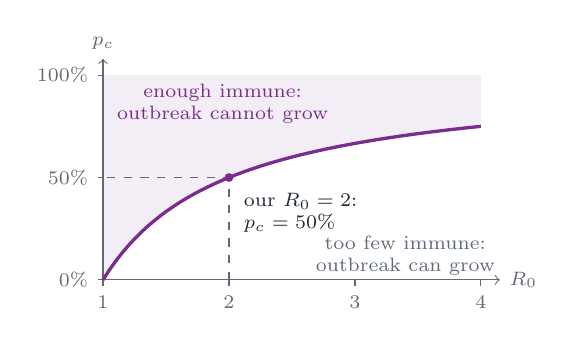
\begin{tikzpicture}[x=1.6cm, y=2.6cm, font=\scriptsize]
    % shaded region: enough immunity, outbreak cannot grow
    \fill[mvSoft] (0,0) -- plot[domain=1:4, samples=60] ({\x-1},{1-1/\x}) -- (3,1) -- (0,1) -- cycle;
    \draw[->, mvInk!70] (0,0) -- (3.15,0) node[right] {$R_0$};
    \draw[->, mvInk!70] (0,0) -- (0,1.08) node[above] {$p_c$};
    \foreach \r in {1,2,3,4} \draw[mvInk!70] ({\r-1},0) -- ({\r-1},-0.03) node[below] {\r};
    \foreach \p/\l in {0/0\%,0.5/50\%,1/100\%} \draw[mvInk!70] (0,\p) -- (-0.04,\p) node[left] {\l};
    \draw[very thick, mvPINN, domain=1:4, samples=60] plot ({\x-1},{1-1/\x});
    \draw[dashed, mvMuted] (1,0) -- (1,0.5) -- (0,0.5);
    \fill[mvPINN] (1,0.5) circle (1.6pt);
    \node[mvInk, anchor=north west, align=left] at (1.04,0.47) {our $R_0 = 2$:\\$p_c = 50\%$};
    \node[mvPINN, align=center] at (0.95,0.86) {enough immune:\\outbreak cannot grow};
    \node[mvMuted, align=center] at (2.4,0.12) {too few immune:\\outbreak can grow};
  \end{tikzpicture}\\[4pt]
  \scriptsize\setlength{\tabcolsep}{6pt}
  \begin{tabular}{@{}lcccc@{}}
    \toprule
    $R_0$ & 1.5 & 2 & 3 & 4 \\
    \midrule
    $p_c = 1 - 1/R_0$ & 33\% & \textbf{50\%} & 67\% & 75\% \\
    \bottomrule
  \end{tabular}
\column{0.51\textwidth}
  \footnotesize\raggedright
  \textbf{\color{mvPINN}Where it comes from}
  \begin{itemize}\setlength{\itemsep}{0pt}
    \item one case infects $R_t = R_0\, s$ people (only susceptible contacts count), so growth stops once $s < 1/R_0$: the immune share must exceed $p_c = 1 - 1/R_0$
    \item same threshold as Module 2: a disease-free state is stable only if $R_0 s^* < 1$
  \end{itemize}
  \textbf{\color{mvPINN}Two ways to reach it}
  \begin{itemize}\setlength{\itemsep}{0pt}
    \item \textbf{immunity}, by vaccination or past infection; there was no licensed Ebola vaccine in 2014--15
    \item \textbf{cutting transmission} by $\delta$: $R_t = (1-\delta) R_0\, s < 1$ when $\delta > \delta_c = 1 - 1/R_0$ (50\% for $R_0 = 2$)
  \end{itemize}
  \textbf{\color{mvPINN}Two subtleties}
  \begin{itemize}\setlength{\itemsep}{0pt}
    \item \textbf{overshoot:} reaching $p_c$ only marks the \emph{peak}; those still infectious keep infecting, so with $R_0 = 2$ about 80\% are infected in the end, not 50\%
    \item \textbf{timing:} later on less is needed, $1 - 1/R_t$: 37.5\% at $s = 0.8$
  \end{itemize}
\end{columns}
\mvTakeaway{\textbf{What it means for control:} without a vaccine, isolation, safe burials and tracing together must cut transmission by \textbf{more than 50\%} at the start, and the earlier they act, the smaller the epidemic.}
\end{frame}
